\documentclass[t]{beamer}
\usetheme{Copenhagen}
\setbeamertemplate{headline}{} % remove toc from headers
\beamertemplatenavigationsymbolsempty

\usepackage{amsmath, tikz, bm, pgfplots, tcolorbox, graphicx}
\pgfplotsset{compat = 1.16}

\title{Measures of Center}
\author{}
\date{}

\AtBeginSection[]
{
  \begin{frame}
    \frametitle{Objectives}
    \tableofcontents[currentsection]
  \end{frame}
}

\begin{document}

\begin{frame} 
\maketitle
\end{frame}

\section{Calculate the mean, median, and mode of a dataset}

\begin{frame}{Measures of Center}
In this section, we will look at finding a central location for a dataset. \newline\\	\pause

In some instances, this can give us a good value to expect from that dataset.
\end{frame}

\begin{frame}{The Mean}
\begin{tcolorbox}[colframe=green!20!black, colback = green!30!white,title=\textbf{Mean}]
The \textbf{mean} of a dataset is found by adding all of the data values together and then dividing by the total number of values. 
\end{tcolorbox}
\vspace{11pt}	\pause

When most people use the term \textit{average}, they are referring to the mean.
\end{frame}

\begin{frame}{Properties of the Mean}
\begin{itemize}
	\item<+-> Sample means drawn from the same population tend to vary less than other measures of center.	\newline\\
	\item<+-> The mean of a data set uses every value, unless the mean is a \textit{trimmed mean}.	\newline\\
	\item<+-> One extreme value (called an {\color{blue}\textbf{outlier}}) can change the value of the mean drastically.	\newline\\
\end{itemize}
\end{frame}

\begin{frame}{Mean Formula}
Sample mean: $\overline{x}$	\qquad	Population mean: $\mu$	\newline\\	\pause
\[ \overline{x}, \text{ or } \mu, = \frac{\sum x_i}{n} = \frac{1}{n}\sum x_i	\]
\end{frame}

\begin{frame}{The Median}

\begin{tcolorbox}[colframe=green!20!black, colback = green!30!white,title=\textbf{Median}]
The \textbf{median} of a dataset is found by first arranging the data values from least to greatest, then selecting the data value in the middle. 
\end{tcolorbox}
\vspace{11pt}	\pause

If there are 2 data values in the middle, the median will be the mean of these two values.
\end{frame}

\begin{frame}{Properties of the Median}
The median separates the top 50\% of the data from the bottom 50\%.	\newline\\	\pause

Unlike, the mean, the median typically does not change by large amounts when we include just a few extreme values; in other words, the median is \textbf{resistant}.	\newline\\	\pause

The median is denoted by $\tilde{x}$, however, some technologies uses \texttt{Med} to denote it.
\end{frame}

\begin{frame}{The Mode}

\begin{tcolorbox}[colframe=green!20!black, colback = green!30!white,title=\textbf{Mode}]
The \textbf{mode} of a dataset is the value(s) that occur the most.
\end{tcolorbox}
\vspace{11pt}	\pause

There may be one mode, no mode, or many modes (2 modes is called \textbf{bimodal}).	\newline\\	\pause

The mode is the only measure of center that is applicable to qualitative data.
\end{frame}

\begin{frame}{Example 1}
The dataset below represents the number of complaints I receive each week about my teaching. \newline\\
\begin{center}
8, 2, 3, 7, 4, 4, 1, 9, 7, 5
\end{center}
\vspace{8pt}

Calculate the mean, median, and mode of the number of complaints.
\end{frame}

\begin{frame}{Example 1}
The total number of complaints is 50. There are 10 complaints listed.	\newline\\	\pause
\begin{center}
Mean = 50/10 = 5 complaints per week.
\end{center}
\vspace{8pt}	\pause

Sorted: 1, 2, 3, 4, 4, 5, 7, 7, 8, 9	\newline\\	\pause
Median number of complaints per week is 4.5	\newline\\	\pause
Mode number of complaints per week are 4 and 7.
\end{frame}

\begin{frame}{Example 2}
The next week, I received 400 complaints. Re-calculate the mean, median, and mode now.	\newline\\	\pause
\begin{center}
1, 2, 3, 4, 4, 5, 7, 7, 8, 9, 400
\end{center}
\vspace{8pt}	\pause

Mean: 450 / 11 = 40.9 complaints per week.	\newline\\	\pause
Median: 5 complaints per week.	\newline\\	\pause
Mode: 4 and 7 complaints per week.
\end{frame}


\section{Calculate the weighted mean of a dataset}

\begin{frame}{Example 3}
California has a mean class size of 20.9 students per teacher and Alaska has a mean of 16.8 students per teacher. \newline\\ 

If we combine the two states, we might find the mean number of students per teacher to be 18.85 (0.5 * (20.9 + 16.8)) but is this result correct? Why or why not?	\newline\\	\pause

It is not correct because California has a much higher population that Alaska. We would have to find what is known as the \textbf{weighted mean}.
\end{frame}

\begin{frame}{Weighted Mean}
Sometimes it is necessary to take into account how large each class of a data set is (such as the population of each US state).	\newline\\	\pause

If $w_i$ represents the {\color{blue}\textbf{weight}} of each class, then the \textbf{weighted mean} can be found via

\[\frac{\sum \left(x_i \cdot w_i\right)}{\sum w_i}\]
\vspace{8pt}	\pause

In other words, \newline\\
\begin{enumerate}
	\item Multiply each data value by its corresponding weight.	\pause
	\item Add those results.	\pause
	\item Then divide that by the total of the weights.
\end{enumerate}
\end{frame}

\begin{frame}{Example 4}
You've recently completed a semester. Determine the semester's GPA (A = 4pts, B = 3pts, etc).	\newline\\
\begin{center}
\begin{tabular}{|c|c|c|}
\textbf{Course} 			&	\textbf{Grade}	&	\textbf{Credit Hours} 	\\	\hline
Statistics					&	A 				&	4						\\
Advanced Chris Farley		&	A 				&	3						\\
\textit{Airplane!} Quotes	&	B 				&	5						\\
Obnoxious Examples			&	C 				&	3						\\
\end{tabular}
\end{center}
\end{frame}

\begin{frame}{Example 4}
\begin{center}
\begin{tabular}{c|c|c}
\textbf{Grade}	&	\textbf{Credit Hours}	&	\textbf{TOTALS} 	\\	\hline
4 				&	4						&	16						\\
4 				&	3						&	12						\\
3 				&	5						&	15						\\
2 				&	3						&	6						\\	\hline
				&	15						&	49					\\
\end{tabular}
\end{center}
\vspace{10pt}	\pause

Weighted Mean: $49/15 = 3.267$
\end{frame}

\begin{frame}{Example 5}
In a statistics course, tests count for 60\% of the final grade, homework for 20\% and midterm and final exams are 10\% each. Suppose you've earned an 87\% average on tests, 94\% average on homeworks and a 77\% average on the exams. \newline\\ 
What is your overall percentage?	\newline\\	\pause
\begin{center}
\begin{tabular}{|c|c|c|c|}
\textbf{Assessment}	&	\textbf{Your Scores}	&	\textbf{Grade Weights}	&	\textbf{TOTALS}	\\	\hline
Tests 				&	0.87					&	0.60					&	0.522			\\
Homework 			&	0.94					&	0.20					&	0.188			\\
Exams 				&	0.77					&	0.20					&	0.154			\\
\end{tabular}
\end{center}
\end{frame}

\begin{frame}{Example 5}
\begin{center}
\begin{tabular}{|c|c|}
\textbf{Grade Weights}	&	\textbf{TOTALS}	\\	\hline
0.60					&	0.522			\\
0.20					&	0.188			\\
0.20					&	0.154			\\	\hline
\onslide<2->{1						&	0.864}			\\
\end{tabular}
\end{center}

\onslide<3->{Grade: $0.864/1 = 86.4\%$}
\end{frame}

\section{Approximate the mean for a grouped dataset}

\begin{frame}{Grouped Data}
When data is presented in its grouped form, we lose out on knowing the individual elements within the dataset. \newline\\	\pause

This means our measures of center, such as mean, can only be our best educated guess.	\newline\\	\pause

We will use similar techniques like we did in finding the weighted mean, however we will have to use the class midpoints as our observed values.
\end{frame}

\begin{frame}{Example 6}
(I swear this is a true story) On one very hungry day of mine, I ordered and consumed 19 sushi rolls from an all-you-can-eat sushi restaurant. This, as you might guess, is not typical (at least for me). The table below indicates the frequencies of sushi rolls I typically eat.	\newline\\
\begin{center}
\begin{tabular}{|c|c|}
\textbf{Number of Rolls} & \textbf{Frequency} \\ \hline
1 -- 5		&	4	\\
6 -- 10		&	17	\\
11 -- 15	&	12	\\
\end{tabular}
\end{center} 

Estimate the mean number of rolls consumed.
\end{frame}

\begin{frame}{Example 6}
\begin{center}
\begin{tabular}{|c|c|c|}
\textbf{Class Midpoint} & \textbf{Frequency}	&	\textbf{TOTALS} \\ \hline
3		&	4	&	12	\\
8		&	17	&	136	\\
13		&	12	&	156 \\	\hline
		&	33	&	304	\\
\end{tabular}
\end{center} 
\vspace{8pt}
\onslide<2->{Mean: $304/33 \approx 9.2$ rolls per visit.}
\end{frame}

\section{Determine if a dataset appears skewed left, skewed right, or normal}

\begin{frame}{Skewness}
When normally distributed (bell-shaped), the mean, median, and mode are (roughly) equal. However, some data sets my be \emph{skewed} (remember, skewness refers to the tail).	\newline\\	\pause

If the mean is (significantly) less than the median, the data is \textbf{skewed left} (or \textbf{negatively skewed}).	
\begin{center}
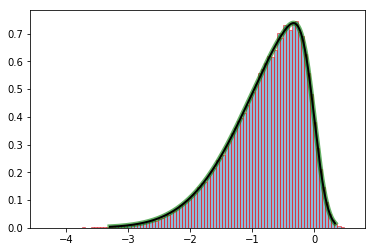
\includegraphics[scale=0.5]{../Images/left_skewed.png}
\end{center}
\end{frame}

\begin{frame}{Skewness}
If the mean is (approximately) equal to the median, the data is \textbf{normal} (no skewness)
\begin{center}
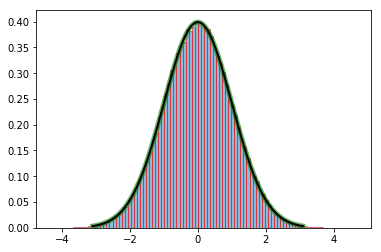
\includegraphics[scale=0.5]{../Images/normal.png}
\end{center}
\end{frame}

\begin{frame}{Skewness}
If the mean is (significantly) greater than the median, the data is \textbf{skewed right} (or \textbf{positively skewed}).
\begin{center}
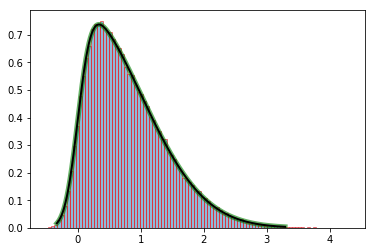
\includegraphics[scale=0.5]{../Images/right_skewed.png}
\end{center}
\end{frame}

\end{document}